\documentclass[twoside,10pt]{article}
\usepackage{amsmath,amsfonts,amsthm,fullpage,amssymb}
%\usepackage{mymath}
\usepackage{algorithm}
\usepackage{algorithmic}
\usepackage{graphicx}
\usepackage{url}
\usepackage{subcaption}




\begin{document}

\title{ISYE 6740 Homework 3\\ 
\small Total 100 points. }
\author{Arjun Singh}
\date{\today}
\maketitle

%----------------------------------------------------------------------------------
\begin{enumerate}

\item {\bf Basic optimization.} (30 points.)

Consider a simplified logistic regression problem. 
Given $m$ training samples $(x_i, y_i)$, $i = 1, \ldots, m$. The data $x_i \in \mathbb R$ (note that we only have one feature for each sample), and $y_i \in \{0, 1\}$.  To fit a logistic regression model for classification, we solve the following optimization problem, where $\theta \in \mathbb R$ is a parameter we aim to find:
\begin{equation}
\max_\theta \ell (\theta), \label{eq:1}
\end{equation}
where the log-likelhood function \[\ell(\theta) = \sum_{i=1}^m \left\{-\log (1+\exp\{-\theta x_i\}) + (y_i-1) \theta x_i\right\}.\]

\begin{enumerate}
\item (10 points) Show step-by-step mathematical derivation for the gradient of the cost function $\ell(\theta)$ in (\ref{eq:1}) and write a pseudo-code  for performing {\bf gradient descent} to find the optimizer $\theta^*$. This is essentially what the training procedure does. (pseudo-code  means you will write down the steps of the algorithm, not necessarily any specific programming language.)\\


\begin{itemize}
\item Answer:  
In order to perform gradient descent, we need to find the gradient of the cost function. In this case, we can differentiate $\ell(\theta)$ w.r.t $\theta$. We can assume $x$ and $y$ to be constants.\\
\[\ell(\theta) = \sum_{i=1}^m \left\{-\log (1+\exp\{-\theta x_i\}) + (y_i-1) \theta x_i\right\}.\]

$$\frac{d\ell(\theta)}{d\theta} = \sum_{i=1}^m \left\{-\frac{1}{1+\exp\{-\theta x_i\}}\cdot \exp\{-\theta x_i\} \cdot -x_i + (y_i-1)x_i\right\}$$

$$\frac{d\ell(\theta)}{d\theta} = \sum_{i=1}^m \left\{\frac{x_i\exp\{-\theta x_i\}}{1+\exp\{-\theta x_i\}} + (y_i-1)x_i\right\} $$

Pseudo code (Algorithm 1):
\begin{itemize}
\item
\begin{algorithm}
\caption{Calculate Pseudo Code for performing Gradient Descent}
\begin{algorithmic}

\STATE Initialize $\theta$ randomly
\STATE Initialize Error $E$ to $\infty$
\STATE Initialize learning rate $\alpha$
\STATE Set error threshold $\epsilon$ to a low value\\
\STATE 
\WHILE{$Error > \epsilon$}
\STATE Calculate the gradients using $\theta_{i}$
\STATE $\theta_{i+1} = \theta_{i} + \alpha \cdot gradient$
\IF {$\theta_{i+1} - \theta_{i} < \epsilon$}
\STATE Stop
\ENDIF

\ENDWHILE
\end{algorithmic}
\end{algorithm}
\end{itemize}








\end{itemize}
\item (10 points) Present a {\bf stochastic gradient descent} algorithm to solve the training of logistic regression problem (\ref{eq:1}). 

\begin{itemize}
\item Stochastic gradient descent involves using a small subset $S_k$ of the data points. This leads to a much faster runtime of the algorithm since not all data points need to be considered for each iteration. In the case of stochastic gradient descent, the gradient of the cost function becomes the following:\\
$$\frac{d\hat{\ell}(\theta)}{d\theta} = \sum_{j \in S_k}^m \sum_{i=1}^m \left\{\frac{x_i\exp\{-\theta x_i\}}{1+\exp\{-\theta x_i\}} + (y_i-1)x_i\right\} $$\\
where each iteration uses a different subset $S_k, k = 1,2,..$

Pseudo code (Algorithm 2):
\begin{itemize}
\item
\begin{algorithm}
\caption{Calculate Pseudo Code for performing Stochastic Gradient Descent}
\begin{algorithmic}

\STATE Initialize $\theta$ randomly
\STATE Initialize Error $E$ to $\infty$
\STATE Initialize learning rate $\alpha$
\STATE Set error threshold $\epsilon$ to a low value\\
\STATE 
\WHILE{$Error > \epsilon$}
\STATE Select random subset $S_k$
\STATE Calculate the gradients on this subset
\STATE $\theta_{i+1} = \theta_{i} + \alpha \cdot gradient$
\IF {$\left\Vert gradient \right\Vert < \epsilon$}
\STATE Stop
\ENDIF

\ENDWHILE
\end{algorithmic}
\end{algorithm}
\end{itemize}

\end{itemize}

\item (10 points) We will {\bf show that the training problem in basic logistic regression problem is concave.} Derive the Hessian matrix of $\ell(\theta)$ and based on this, show the training problem (\ref{eq:1}) is concave (note that in this case, since we only have one feature, the Hessian matrix is just a scalar). Explain why the problem can be solved efficiently and gradient descent will achieve a unique global optimizer, as we discussed in class. 

\begin{itemize}
\item Answer:\\
In order to show that the training problem is concave, we need to prove that the second derivative of the cost function is negative.
$$\frac{d\ell(\theta)}{d\theta} = \sum_{i=1}^m \left\{\frac{x_i\exp\{-\theta x_i\}}{1+\exp\{-\theta x_i\}} + (y_i-1)x_i\right\} $$

$$\frac{d^2\ell(\theta)}{d\theta^2} = \sum_{i=1}^m \left\{\frac{-x_i^2\exp\{-\theta x_i\}(1+\exp\{-\theta x_i\}) + x_i^2exp\{-2\theta x_i\}}{(1+\exp\{-\theta x_i\})^2} \right\} $$

$$\frac{d^2\ell(\theta)}{d\theta^2} = \sum_{i=1}^m \left\{\frac{-x_i^2\exp\{-\theta x_i\}}{(1+\exp\{-\theta x_i\})^2} \right\} $$

The negative sign on the Hessian proves that the function is concave. Since the function is concave over the entire domain, it can be solved efficiently as there is only 1 global optimum.

\end{itemize}

\end{enumerate}
 
\item {\bf Comparing Bayes, logistic, and KNN classifiers.} (30 points)

In lectures we learn three different classifiers. This question is to implement and compare them. We are suggest use \textsf{Scikit-learn}, which is a commonly-used and powerful \textsf{Python} library with various machine learning tools. But you can also use other similar library in other languages of your choice to perform the tasks. 




\textbf{Part One (Divorce classification/prediction).} (20 points) 

This dataset is about participants who completed the personal information form and a divorce predictors scale. 

The data is a modified version of the publicly available at \url{https://archive.ics.uci.edu/ml/datasets/Divorce+Predictors+data+set} (by injecting noise so you will not replicate the results on uci website). There are 170 participants and 54 attributes (or predictor variables) that are all real-valued. The dataset \textbf{marriage.csv}. The last column of the CSV file is label $y$ (1 means ``divorce'', 0 means ``no divorce''). Each column is for one feature (predictor variable), and each row is a sample (participant). A detailed explanation for each feature (predictor variable) can be found at the website link above. Our goal is to build a classifier using training data, such that given a test sample, we can classify (or essentially predict) whether its label is 0 (``no divorce'') or 1 (``divorce''). 



Build three classifiers using ({\bf Naive Bayes, Logistic Regression, KNN}). Use the first $80\%$ data for training and the remaining $20\%$ for testing. If you use \textsf{scikit-learn} you can use \textsf{train\_test\_split} to split the dataset. 

\textit{Remark: Please note that, here, for Naive Bayes, this means that we have to estimate the variance for each individual feature from training data. When estimating the variance, if the variance is zero to close to zero (meaning that there is very little variability in the feature), you can set the variance to be a small number, e.g., $\epsilon = 10^{-3}$. We do not want to have include zero or nearly variance in Naive Bayes. This tip holds for both Part One and Part Two of this question.}

\begin{enumerate}

	\item (10 points) Report testing accuracy for each of the three classifiers.  Comment on their performance: which performs the best and make a guess why they perform the best in this setting. 
	
	\begin{itemize}
	\item Answer:\\
	After training the three classifiers, here are the results I achieved:\\
	The accuracy of the Naive Bayes classifier is 94.12\%\\
	The accuracy of the Logistic Regression classifier is 91.18\%\\
	The accuracy of the K Nearest Neighbours classifier is 94.12\%\\
	 I perfomed multiple runs, and in most cases, the Naive Bayers classifier and the KNN classifier performed similarly, giving better performance as compared to the Logistic Regression classifier.\\
	 
	 One explanation for a better performance by the Naive Bayes classifier over the Logistic Regression is that it is a generative model that reaches its asymptotic solution faster (i.e. with fewer training points) as compared to Logistic Regression, which is a discriminative model and takes longer to reach its solution. Since the training dataset is fairly small (170 data points), this makes sense, however, with larger datasets, it is expected that the Logistic Regression model would outperform the Naive Bayes model.\\
	 
	 Reference:\url{https://medium.com/@sangha_deb/naive-bayes-vs-logistic-regression-a319b07a5d4c#:~:text=Naive%20Bayes%20also%20assumes%20that,will%20be%20a%20better%20classifier}\\
	 
	 Similarly, the KNN classifier performs well in this case as it is able to fit to non-linear problems and is non-parametric.
	\end{itemize}
	\item (10 points) Use the first two features to train three new classifiers. Plot the data points and decision boundary of each classifier. Comment on the difference between the decision boundary for the three classifiers. Please clearly represent the data points with different labels using different colors.
	\begin{itemize}
	\item Answer:\\
	Using only the first two features, we get the following accuracies for the classifiers:\\
	The accuracy of the Naive Bayes classifier is 85.29\%\\
	The accuracy of the Logistic Regression classifier is 82.35\%\\
	The accuracy of the K Nearest Neighbours classifier is 85.29\%\\
	
	The results were similar across multiple trials. In general, the accuracy of the models is less since there are fewer features to train on. The decision boundaries for the classifiers can be seen in Figure 1.\\
	Since this implementation of Naive Bayes used the Gaussian, the decision boundary is quadratic. The Logistic Regression has a linear decision boundary and the KNN classifier has a non-linear boundary.
	
\begin{figure}
\begin{subfigure}{.3\textwidth}
  \centering
  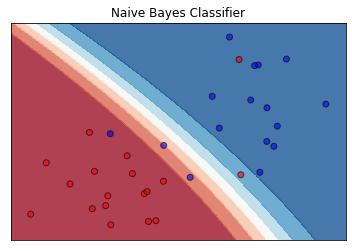
\includegraphics[width=.8\linewidth]{NBDecisionBoundary.png}
  \caption{Naive Bayes Classifier}
  \label{fig:sfig1}
\end{subfigure}%
\begin{subfigure}{.3\textwidth}
  \centering
  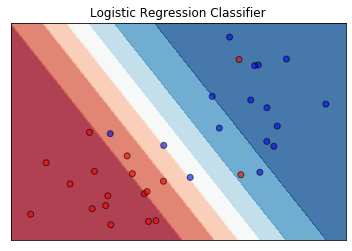
\includegraphics[width=.8\linewidth]{LRDecisionBoundary.png}
  \caption{Logistic Regression Classifier}
  \label{fig:sfig2}
\end{subfigure}
\begin{subfigure}{.3\textwidth}
  \centering
  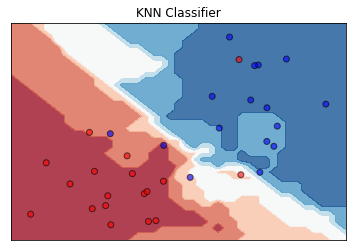
\includegraphics[width=.8\linewidth]{KNNDecisionBoundary.png}
  \caption{KNN Classifier}
  \label{fig:sfig2}
\end{subfigure}
\caption{Decision Boundaries}
\label{fig:fig}
\end{figure}
	
	\end{itemize}
\end{enumerate}

\textbf{Part Two (Handwritten digits classification).} (10 points) Repeat the above using the \textbf{MNIST Data} in our \textbf{Homework 2}. Here, give ``digit'' 6 label $y = 1$, and give ``digit'' 2 label $y = 0$. All the pixels in each image will be the feature (predictor variables) for that sample (i.e., image). Our goal is to build classifier to such that given a new test sample, we can tell is it a 2 or a 6. Using the first $80\%$ of the samples for training and remaining $20\%$ for testing. Report the classification accuracy on testing data, for each of the three classifiers. Comment on their performance: which performs the best and make a guess why they perform the best in this setting. 
\begin{itemize}
\item Answer:\\
Using the MNIST dataset from the previous homework, the classifier accuracies were as follows:\\
The accuracy of the Naive Bayes classifier is 76.13\%\\
The accuracy of the Logistic Regression classifier is 97.49\%\\
The accuracy of the K Nearest Neighbours classifier is 99.75\%\\

In this case, the KNN classifier performed the best since the images have many features and are non-parametric, making it an ideal problem for non-linear methods like KNN. The Logistic regression also performed fairly well and it can be attributed to the fact that there is significant amount of data available to train on. Naive Bayes on the other hand is unable to handle such classification problems nearly as well as the other classifiers.

\end{itemize}


\item {\bf Naive Bayes for spam filtering}. (40 points) %(Bonus question: 20 points) 

In this problem we will use the Naive Bayes algorithm to fit a spam filter by hand. This will enhance your understanding to Bayes classifier and build intuition. This question does not involve any programming but only derivation and hand calculation. 

Spam filters are used in all email services to classify received emails as ``Spam'' or ``Not Spam''. A simple approach involves maintaining a vocabulary of words that commonly occur in ``Spam'' emails and classifying an email as ``Spam'' if the number of words from the dictionary that are present in the email is over a certain threshold.
We are given the vocabulary consists of 15 words \[V=\{\textsf{secret, offer, low, price, valued, customer, today, dollar, million, sports, is, for, play, healthy, pizza}\}.\] We will use $V_i$ to represent the $i$th word in $V$. As our training dataset, we are also given 3 example spam messages,
\begin{itemize}
\item \textsf{million dollar offer}
\item \textsf{secret offer today}
\item \textsf{secret is secret}
\end{itemize}
and 4 example non-spam messages
\begin{itemize}
\item \textsf{low price for valued customer}
\item \textsf{play secret sports today}
\item \textsf{sports is healthy}
\item \textsf{low price pizza}
\end{itemize}

Recall that the Naive Bayes classifier assumes the probability of an input depends on its input feature. The feature for each sample is defined as
$x^{(i)} = [x_1^{(i)}, x_2^{(i)}, \ldots, x_d^{(i)}]^T$, $i = 1, \ldots, m$ and the class of the $i$th sample is $y^{(i)}$. In our case the length of the input vector is $d = 15$, which is equal to the number of words in the vocabulary $V$. Each entry $x_j^{(i)}$ is equal to the number of times word $V_j$ occurs in the $i$-th message. %The marginal distribution of 

\begin{enumerate}
\item (5 points) Calculate class prior $\mathbb P(y = 0)$ and $\mathbb P(y = 1)$ from the training data, where $y = 0$ corresponds to spam messages, and $y = 1$ corresponds to non-spam messages. Note that these class prior essentially corresponds to the frequency of each class in the training sample. 
\begin{itemize}
\item Answer:\\
Since we have 3 spam messages and 4 non-spam messages, the $\mathbb P(y = 0)= \frac{3}{7}$ and  $\mathbb P(y = 1) = \frac{4}{7}$
\end{itemize}
\item (10 points) Write down the feature vectors for each spam and non-spam messages.
\begin{itemize}
\item Answer:\\
The feature vectors can be calculated by computing the frequency of the words in $V$ for each of the 7 messages. This can be seen in Figure 2.

\begin{figure}[h!]
\begin{center}
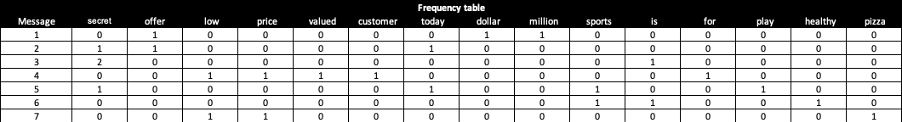
\includegraphics[totalheight=0.8in]{Q3bFrequencyTable.png}
\end{center}
\caption{Feature Vectors for Each Message}
\end{figure}

\end{itemize}

\item (15 points) In the Naive Bayes model, assuming the keywords are independent of each other (this is a simplification), the likelihood of a sentence with its feature vector $x$ given a class $c$ is given by 
\[
\mathbb P (x|y = c) = \prod_{k=1}^d \theta_{c, k}^{x_k}, \quad c = \{0, 1\}
\]
where $0 \leq \theta_{c,k} \leq 1$ is the probability of word $k$ appearing in class $c$, which satisfies 
\[\sum_{k=1}^d \theta_{c, k} = 1, \quad \forall c.\] Given this, the complete log-likelihood function for our training data is given by
\[
\ell(\theta_{1,1}, \ldots, \theta_{1, d}, \theta_{2,1}, \ldots, \theta_{2, d}) = 
\sum_{i=1}^m \sum_{k=1}^d x_k^{(i)} \log \theta_{y^{(i)}, k}
\]
(In this example, $m = 7$.)
 Calculate the maximum likelihood estimates of $\theta_{0,1}$, $\theta_{0,7}$, $\theta_{1,1}$, $\theta_{1,15}$ by maximizing the log-likelihood function above.
 %$\mathbb P (x|y = c)$ with respect to $\theta_{c, k}$ and given data. 
 (Hint: We are solving a constrained maximization problem. To do this, remember, you  need to introduce two Lagrangian multiplier because you have two constraints.)
\begin{itemize}
\item Answer:\\
We are given the constraints:
$$\sum_{k=1}^d \theta_{0, k} = 1 $$
$$\sum_{k=1}^d \theta_{1, k} = 1 $$
We can introduce 2 Lagrangian multipliers to solve the following problem:
$$g(\lambda,\theta) = \sum_{i=1}^m \sum_{k=1}^d x_k^{(i)} \log \theta_{y^{(i)}, k} - \lambda(\theta_{y^{(i)}, k} - 1)$$	where $y = 0$ for spam and $y=1$ for non-spam messages.\\
We can find the solution to his problem by setting:
$$\frac{d}{d\theta_{y,k}}g(\lambda,\theta_{y,k}) = 0$$
$$\frac{d}{d\theta_{y,k}}g(\lambda,\theta_{y,k}) = \frac{x_k}{\theta_{y,k}} - \lambda $$

$$\theta_{y,k} = \frac{x_k}{\lambda}$$
Incorporating the constraints, we get:
$$\theta_{y,k} = \frac{x_k}{\sum_{k=1}^d x_k}$$

From this result, we can compute:\\
$$\theta_{0,1} = \frac{3}{9} $$
$$\theta_{0,7} = \frac{1}{9} $$

$$\theta_{1,1} = \frac{1}{15} $$
$$\theta_{1,15} = \frac{1}{15} $$\\




\end{itemize} 
 
\item (10 points) Given a test message ``\textsf{today is secret}'', using the Naive Bayes classier that you have trained in Part (a)-(c), to calculate the posterior and decide whether it is spam or not spam.
\begin{itemize}
\item Answer:\\
To decide whether ``\textsf{today is secret}'' is spam or not, we can calculate the posteriors in the following manner:\\
Let $m = ``\textsf{today is secret}''$\\
Then
$$
\mathbb P (spam|m) = \frac{P (m|spam) \cdot P (spam)}{P (m)}
$$

$$
\mathbb P (spam|m) = \frac{\frac{1}{9} \cdot \frac{1}{9} \cdot \frac{3}{9} \cdot \frac{3}{7}}{\frac{1}{9} \cdot \frac{1}{9} \cdot \frac{3}{9} \cdot \frac{3}{7} + \frac{1}{15} \cdot \frac{1}{15} \cdot \frac{1}{15} \cdot \frac{4}{7}}
$$

$$
\mathbb P (spam|m) = 0.9124
$$
Similarly, for classifying if the message is not spam:

$$
\mathbb P (not spam|m) = \frac{P (m|not spam) \cdot P (not spam)}{P (m)}
$$

$$
\mathbb P (not spam|m) = \frac{\frac{1}{15} \cdot \frac{1}{15} \cdot \frac{1}{15} \cdot \frac{4}{7}}{\frac{1}{9} \cdot \frac{1}{9} \cdot \frac{3}{9} \cdot \frac{3}{7} + \frac{1}{15} \cdot \frac{1}{15} \cdot \frac{1}{15} \cdot \frac{4}{7}}
$$

$$
\mathbb P (not spam|m) = 0.0876
$$

Taking the log-likelihood ratio:
$$
-ln \left(\frac{0.9124}{0.0876}\right) = -2.34
$$
Since the ratio is $<$ 0, the message is classified as spam.


\begin{figure}[h!]
\begin{center}
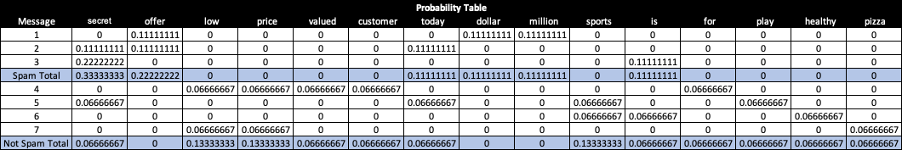
\includegraphics[totalheight=1in]{Q3ProbabilityTable.png}
\end{center}
\caption{Probability Table Used For Calculations}
\end{figure}

\end{itemize}

\end{enumerate}


\end{enumerate}


\end{document}
